% Options for packages loaded elsewhere
\PassOptionsToPackage{unicode}{hyperref}
\PassOptionsToPackage{hyphens}{url}
\PassOptionsToPackage{dvipsnames,svgnames,x11names}{xcolor}
\documentclass[
]{article}
\usepackage{xcolor}
\usepackage[margin=1in]{geometry}
\usepackage{amsmath,amssymb}
\setcounter{secnumdepth}{-\maxdimen} % remove section numbering
\usepackage{iftex}
\ifPDFTeX
  \usepackage[T1]{fontenc}
  \usepackage[utf8]{inputenc}
  \usepackage{textcomp} % provide euro and other symbols
\else % if luatex or xetex
  \usepackage{unicode-math} % this also loads fontspec
  \defaultfontfeatures{Scale=MatchLowercase}
  \defaultfontfeatures[\rmfamily]{Ligatures=TeX,Scale=1}
\fi
\usepackage{lmodern}
\ifPDFTeX\else
  % xetex/luatex font selection
\fi
% Use upquote if available, for straight quotes in verbatim environments
\IfFileExists{upquote.sty}{\usepackage{upquote}}{}
\IfFileExists{microtype.sty}{% use microtype if available
  \usepackage[]{microtype}
  \UseMicrotypeSet[protrusion]{basicmath} % disable protrusion for tt fonts
}{}
\makeatletter
\@ifundefined{KOMAClassName}{% if non-KOMA class
  \IfFileExists{parskip.sty}{%
    \usepackage{parskip}
  }{% else
    \setlength{\parindent}{0pt}
    \setlength{\parskip}{6pt plus 2pt minus 1pt}}
}{% if KOMA class
  \KOMAoptions{parskip=half}}
\makeatother
\usepackage{color}
\usepackage{fancyvrb}
\newcommand{\VerbBar}{|}
\newcommand{\VERB}{\Verb[commandchars=\\\{\}]}
\DefineVerbatimEnvironment{Highlighting}{Verbatim}{commandchars=\\\{\}}
% Add ',fontsize=\small' for more characters per line
\usepackage{framed}
\definecolor{shadecolor}{RGB}{248,248,248}
\newenvironment{Shaded}{\begin{snugshade}}{\end{snugshade}}
\newcommand{\AlertTok}[1]{\textcolor[rgb]{0.94,0.16,0.16}{#1}}
\newcommand{\AnnotationTok}[1]{\textcolor[rgb]{0.56,0.35,0.01}{\textbf{\textit{#1}}}}
\newcommand{\AttributeTok}[1]{\textcolor[rgb]{0.13,0.29,0.53}{#1}}
\newcommand{\BaseNTok}[1]{\textcolor[rgb]{0.00,0.00,0.81}{#1}}
\newcommand{\BuiltInTok}[1]{#1}
\newcommand{\CharTok}[1]{\textcolor[rgb]{0.31,0.60,0.02}{#1}}
\newcommand{\CommentTok}[1]{\textcolor[rgb]{0.56,0.35,0.01}{\textit{#1}}}
\newcommand{\CommentVarTok}[1]{\textcolor[rgb]{0.56,0.35,0.01}{\textbf{\textit{#1}}}}
\newcommand{\ConstantTok}[1]{\textcolor[rgb]{0.56,0.35,0.01}{#1}}
\newcommand{\ControlFlowTok}[1]{\textcolor[rgb]{0.13,0.29,0.53}{\textbf{#1}}}
\newcommand{\DataTypeTok}[1]{\textcolor[rgb]{0.13,0.29,0.53}{#1}}
\newcommand{\DecValTok}[1]{\textcolor[rgb]{0.00,0.00,0.81}{#1}}
\newcommand{\DocumentationTok}[1]{\textcolor[rgb]{0.56,0.35,0.01}{\textbf{\textit{#1}}}}
\newcommand{\ErrorTok}[1]{\textcolor[rgb]{0.64,0.00,0.00}{\textbf{#1}}}
\newcommand{\ExtensionTok}[1]{#1}
\newcommand{\FloatTok}[1]{\textcolor[rgb]{0.00,0.00,0.81}{#1}}
\newcommand{\FunctionTok}[1]{\textcolor[rgb]{0.13,0.29,0.53}{\textbf{#1}}}
\newcommand{\ImportTok}[1]{#1}
\newcommand{\InformationTok}[1]{\textcolor[rgb]{0.56,0.35,0.01}{\textbf{\textit{#1}}}}
\newcommand{\KeywordTok}[1]{\textcolor[rgb]{0.13,0.29,0.53}{\textbf{#1}}}
\newcommand{\NormalTok}[1]{#1}
\newcommand{\OperatorTok}[1]{\textcolor[rgb]{0.81,0.36,0.00}{\textbf{#1}}}
\newcommand{\OtherTok}[1]{\textcolor[rgb]{0.56,0.35,0.01}{#1}}
\newcommand{\PreprocessorTok}[1]{\textcolor[rgb]{0.56,0.35,0.01}{\textit{#1}}}
\newcommand{\RegionMarkerTok}[1]{#1}
\newcommand{\SpecialCharTok}[1]{\textcolor[rgb]{0.81,0.36,0.00}{\textbf{#1}}}
\newcommand{\SpecialStringTok}[1]{\textcolor[rgb]{0.31,0.60,0.02}{#1}}
\newcommand{\StringTok}[1]{\textcolor[rgb]{0.31,0.60,0.02}{#1}}
\newcommand{\VariableTok}[1]{\textcolor[rgb]{0.00,0.00,0.00}{#1}}
\newcommand{\VerbatimStringTok}[1]{\textcolor[rgb]{0.31,0.60,0.02}{#1}}
\newcommand{\WarningTok}[1]{\textcolor[rgb]{0.56,0.35,0.01}{\textbf{\textit{#1}}}}
\usepackage{graphicx}
\makeatletter
\newsavebox\pandoc@box
\newcommand*\pandocbounded[1]{% scales image to fit in text height/width
  \sbox\pandoc@box{#1}%
  \Gscale@div\@tempa{\textheight}{\dimexpr\ht\pandoc@box+\dp\pandoc@box\relax}%
  \Gscale@div\@tempb{\linewidth}{\wd\pandoc@box}%
  \ifdim\@tempb\p@<\@tempa\p@\let\@tempa\@tempb\fi% select the smaller of both
  \ifdim\@tempa\p@<\p@\scalebox{\@tempa}{\usebox\pandoc@box}%
  \else\usebox{\pandoc@box}%
  \fi%
}
% Set default figure placement to htbp
\def\fps@figure{htbp}
\makeatother
\setlength{\emergencystretch}{3em} % prevent overfull lines
\providecommand{\tightlist}{%
  \setlength{\itemsep}{0pt}\setlength{\parskip}{0pt}}
\usepackage{bookmark}
\IfFileExists{xurl.sty}{\usepackage{xurl}}{} % add URL line breaks if available
\urlstyle{same}
\hypersetup{
  pdftitle={STAT 442/842, CM 762 W25 Assignment 3},
  colorlinks=true,
  linkcolor={Maroon},
  filecolor={Maroon},
  citecolor={Blue},
  urlcolor={blue},
  pdfcreator={LaTeX via pandoc}}

\title{STAT 442/842, CM 762 W25 Assignment 3}
\usepackage{etoolbox}
\makeatletter
\providecommand{\subtitle}[1]{% add subtitle to \maketitle
  \apptocmd{\@title}{\par {\large #1 \par}}{}{}
}
\makeatother
\subtitle{DUE: Friday March 7 by 11:59pm EST}
\author{}
\date{\vspace{-2.5em}}

\begin{document}
\maketitle

\subsection{NOTES}\label{notes}

This assignment has 9 questions for everyone, there are no Manim
questions for grad students.

Your assignment must be submitted by the due date listed at the top of
this document, and it must be submitted electronically in .pdf format
via Crowdmark.

This means that your responses for different question parts should begin
on separate pages of your .pdf file. Note that your .pdf solution file
must have been generated by R Markdown. Additionally:

Organization and comprehensibility is part of a full solution.
Consequently, points will be deducted for solutions that are not
organized and incomprehensible. Furthermore, if you submit your
assignment to Crowdmark, but you do so incorrectly in any way (e.g., you
upload your Question 2 solution in the Question 1 box), you will receive
a 5\% deduction (i.e., 5\% of the assignment's point total will be
deducted from your point total).

There are 30 possible marks for all students. That's 30 each, not 30 to
share between you all.

\newpage

\section{Part 1: Generative Art}\label{part-1-generative-art}

\textbf{Q1) (2 marks)} Using a function from the \texttt{RColorBrewer}
package, make a palette of 60 hexcodes that interpolates linearly, with
default bias and 100\% opacity, through white, royalblue, black,
firebrick, and forestgreen.

Call this palette \texttt{pal\_magic} and report the first seven
hexcodes.

\begin{Shaded}
\begin{Highlighting}[]
\FunctionTok{library}\NormalTok{(RColorBrewer)}

\CommentTok{\#Create the palette using colorRampPalette}
\NormalTok{pal\_magic }\OtherTok{=} \FunctionTok{colorRampPalette}\NormalTok{(}\FunctionTok{c}\NormalTok{(}\StringTok{"white"}\NormalTok{, }\StringTok{"royalblue"}\NormalTok{, }\StringTok{"black"}\NormalTok{, }\StringTok{"firebrick"}\NormalTok{, }\StringTok{"forestgreen"}\NormalTok{))(}\DecValTok{60}\NormalTok{)}

\CommentTok{\#show the first seven hexcodes}
\NormalTok{pal\_magic[}\DecValTok{1}\SpecialCharTok{:}\DecValTok{7}\NormalTok{]}
\end{Highlighting}
\end{Shaded}

\begin{verbatim}
## [1] "#FFFFFF" "#F2F4FC" "#E5EAFA" "#D8E0F8" "#CBD6F6" "#BECCF4" "#B1C1F2"
\end{verbatim}

\begin{Shaded}
\begin{Highlighting}[]
\CommentTok{\#show the entire palette in a plot to confirm the colours}
\FunctionTok{plot}\NormalTok{(}\DecValTok{1}\SpecialCharTok{:}\DecValTok{60}\NormalTok{, }\FunctionTok{rep}\NormalTok{(}\DecValTok{1}\NormalTok{, }\DecValTok{60}\NormalTok{), }\AttributeTok{col =}\NormalTok{ pal\_magic, }\AttributeTok{pch =} \DecValTok{19}\NormalTok{, }\AttributeTok{cex =} \DecValTok{2}\NormalTok{, }\AttributeTok{xlab =} \StringTok{"Index"}\NormalTok{, }\AttributeTok{ylab =} \StringTok{"Color"}\NormalTok{, }\AttributeTok{main =} \StringTok{"pal\_magic"}\NormalTok{)}
\end{Highlighting}
\end{Shaded}

\pandocbounded{
\includegraphics[keepaspectratio]{STAT442_W25_Assignment3_files/figure-latex/unnamed-chunk-1-1.pdf}}

\vspace{5cm}

\newpage

\textbf{Q2) (2 marks)} Using the aRsty package (See
\url{https://github.com/koenderks/aRtsy} for more guidance), draw a
watercolor using \texttt{pal\_magic}, 1 layer, default depth, a grey75
background, and 50 resolution.

\begin{Shaded}
\begin{Highlighting}[]
\FunctionTok{library}\NormalTok{(aRtsy)}
\end{Highlighting}
\end{Shaded}

\begin{verbatim}
## Warning: package 'aRtsy' was built under R version 4.4.2
\end{verbatim}

\begin{Shaded}
\begin{Highlighting}[]
\CommentTok{\#Draw the watercolor}
\FunctionTok{canvas\_watercolors}\NormalTok{(}\AttributeTok{colors =}\NormalTok{ pal\_magic, }\AttributeTok{layers =} \DecValTok{1}\NormalTok{, }\AttributeTok{background =} \StringTok{"grey75"}\NormalTok{, }\AttributeTok{resolution =} \DecValTok{50}\NormalTok{)}
\end{Highlighting}
\end{Shaded}

\pandocbounded{
\includegraphics[keepaspectratio]{STAT442_W25_Assignment3_files/figure-latex/unnamed-chunk-2-1.pdf}}

\vspace{5cm}

\newpage

\textbf{Q3) (4 marks)} Using \texttt{pal\_magic}, the
\texttt{mandelbrot} package, \texttt{geom\_raster},
\texttt{theme\_void}, and \texttt{scale\_fill\_gradientn}, construct an
image on a mandelbrot set. The image should be 600 pixels wide, 400
pixels tall, and include a non-trival portion of the set (that is, not
all divergent and not all convergent). The x and y limits need to be
0.001 across or less.

\begin{Shaded}
\begin{Highlighting}[]
\FunctionTok{library}\NormalTok{(mandelbrot)}
\end{Highlighting}
\end{Shaded}

\begin{verbatim}
## Warning: package 'mandelbrot' was built under R version 4.4.2
\end{verbatim}

\begin{Shaded}
\begin{Highlighting}[]
\FunctionTok{library}\NormalTok{(ggplot2)}
\end{Highlighting}
\end{Shaded}

\begin{verbatim}
## Warning: package 'ggplot2' was built under R version 4.4.1
\end{verbatim}

\begin{Shaded}
\begin{Highlighting}[]
\CommentTok{\#Create the Mandelbrot set}
\NormalTok{mb }\OtherTok{\textless{}{-}} \FunctionTok{mandelbrot}\NormalTok{(}\AttributeTok{xlim =} \FunctionTok{c}\NormalTok{(}\SpecialCharTok{{-}}\FloatTok{0.7435}\NormalTok{, }\SpecialCharTok{{-}}\FloatTok{0.7425}\NormalTok{),}
                 \AttributeTok{ylim =} \FunctionTok{c}\NormalTok{(}\FloatTok{0.131}\NormalTok{, }\FloatTok{0.132}\NormalTok{),}
                 \AttributeTok{resolution =} \FunctionTok{list}\NormalTok{(}\AttributeTok{x =} \DecValTok{600}\NormalTok{, }\AttributeTok{y =} \DecValTok{400}\NormalTok{),}
                 \AttributeTok{iterations =} \DecValTok{1000}\NormalTok{)}

\NormalTok{mandelbrot\_df }\OtherTok{\textless{}{-}} \FunctionTok{data.frame}\NormalTok{(mb)}

\CommentTok{\#Create the ggplot}
\FunctionTok{ggplot}\NormalTok{(mandelbrot\_df, }\FunctionTok{aes}\NormalTok{(}\AttributeTok{x =}\NormalTok{ x, }\AttributeTok{y =}\NormalTok{ y, }\AttributeTok{fill =}\NormalTok{ value)) }\SpecialCharTok{+}
  \FunctionTok{geom\_raster}\NormalTok{(}\AttributeTok{interpolate=}\ConstantTok{TRUE}\NormalTok{) }\SpecialCharTok{+}
  \FunctionTok{theme\_void}\NormalTok{() }\SpecialCharTok{+}
  \FunctionTok{scale\_fill\_gradientn}\NormalTok{(}\AttributeTok{colours =}\NormalTok{ pal\_magic) }
\end{Highlighting}
\end{Shaded}

\pandocbounded{
\includegraphics[keepaspectratio]{STAT442_W25_Assignment3_files/figure-latex/unnamed-chunk-3-1.pdf}}

\newpage

\section{Part 2: Financial Data}\label{part-2-financial-data}

\textbf{Q4) (6 marks)} Using the \texttt{tidyquant} package, make a
chart of the closing stock price for every trading day from Jan 1, 2024
to Jan 1, 2025 of the company ``Spinmaster Toys''. (Hint: Ticker symbols
on the Toronto Stock Exchange end in \texttt{.TO}).

The y limits should be 10\% above and below the maximum and minimum
stock prices within the year, respectively.

If the closing price in Jan 1, 2025 is higher than in Jan 1, 2024 make
the area under the line forestgreen at 50\% opacity, otherwise make the
firebrick at 50\% opacity.

\begin{Shaded}
\begin{Highlighting}[]
\FunctionTok{library}\NormalTok{(tidyquant)}
\FunctionTok{library}\NormalTok{(ggplot2)}
\FunctionTok{library}\NormalTok{(dplyr)}

\CommentTok{\#Ticker symbol for Spinmaster Toys is TOY.TO}

\CommentTok{\# Get the stock data}
\NormalTok{stock\_data }\OtherTok{\textless{}{-}} \FunctionTok{tq\_get}\NormalTok{(}\StringTok{"TOY.TO"}\NormalTok{, }\AttributeTok{from =} \StringTok{"2024{-}01{-}01"}\NormalTok{, }\AttributeTok{to =} \StringTok{"2025{-}01{-}01"}\NormalTok{)}

\CommentTok{\# Define the color of the area under the line}
\NormalTok{fill\_colour }\OtherTok{\textless{}{-}} \ControlFlowTok{if}\NormalTok{ (stock\_data}\SpecialCharTok{$}\NormalTok{close[}\FunctionTok{nrow}\NormalTok{(stock\_data)] }\SpecialCharTok{\textgreater{}}\NormalTok{ stock\_data}\SpecialCharTok{$}\NormalTok{close[}\DecValTok{1}\NormalTok{]) \{}
  \StringTok{"forestgreen"}
\NormalTok{\} }\ControlFlowTok{else}\NormalTok{ \{}
  \StringTok{"firebrick"}
\NormalTok{\}}

\CommentTok{\# Create the plot}
\FunctionTok{ggplot}\NormalTok{(stock\_data, }\FunctionTok{aes}\NormalTok{(}\AttributeTok{x =}\NormalTok{ date, }\AttributeTok{y =}\NormalTok{ close)) }\SpecialCharTok{+}
  \FunctionTok{geom\_line}\NormalTok{(}\AttributeTok{color =} \StringTok{"black"}\NormalTok{) }\SpecialCharTok{+}
  \FunctionTok{geom\_ribbon}\NormalTok{(}\FunctionTok{aes}\NormalTok{(}\AttributeTok{ymin=}\FunctionTok{min}\NormalTok{(close) }\SpecialCharTok{*} \FloatTok{0.9}\NormalTok{, }
                  \AttributeTok{ymax=}\NormalTok{close),}
                  \AttributeTok{fill =}\NormalTok{ fill\_colour,}
                  \AttributeTok{alpha =} \FloatTok{0.5}\NormalTok{) }\SpecialCharTok{+}
  \FunctionTok{ylim}\NormalTok{(}\FunctionTok{min}\NormalTok{(stock\_data}\SpecialCharTok{$}\NormalTok{close) }\SpecialCharTok{*} \FloatTok{0.9}\NormalTok{, }\FunctionTok{max}\NormalTok{(stock\_data}\SpecialCharTok{$}\NormalTok{close) }\SpecialCharTok{*} \FloatTok{1.1}\NormalTok{) }\SpecialCharTok{+}
  \FunctionTok{labs}\NormalTok{(}\AttributeTok{title =} \StringTok{"Spinmaster Toys Stock Price"}\NormalTok{, }\AttributeTok{x =} \StringTok{"Date"}\NormalTok{, }\AttributeTok{y =} \StringTok{"Closing Price"}\NormalTok{) }\SpecialCharTok{+}
  \FunctionTok{theme\_minimal}\NormalTok{()}
\end{Highlighting}
\end{Shaded}

\pandocbounded{
\includegraphics[keepaspectratio]{STAT442_W25_Assignment3_files/figure-latex/unnamed-chunk-4-1.pdf}}

\newpage

\section{Part 3: Network
Visualization}\label{part-3-network-visualization}

\textbf{Q5) (5 marks)} The dataset \texttt{flo} in the \texttt{network}
package is a network of marriages between elite families in Florence,
Italy in the 1200's through the 1400's. After loading the
\texttt{network} package, you can load this dataset with
\texttt{data(flo)}.

See \url{https://briatte.github.io/ggnetwork/articles/ggnetwork.html}
for more guidance.

Draw a network with edges, nodes, and nodetext of \texttt{flo} arranged
in a \texttt{circle} layout. Label the nodes with the names of the
families, in \texttt{firebrick} color and a bold font face. Use
\texttt{theme\_blank()}.

\begin{Shaded}
\begin{Highlighting}[]
\FunctionTok{library}\NormalTok{(ggnetwork)}
\FunctionTok{library}\NormalTok{(network)}
\FunctionTok{library}\NormalTok{(sna)}

\CommentTok{\# Load the dataset}
\FunctionTok{data}\NormalTok{(flo)}

\NormalTok{flo }\OtherTok{\textless{}{-}} \FunctionTok{network}\NormalTok{(flo, }\AttributeTok{directed =} \ConstantTok{FALSE}\NormalTok{)}


\CommentTok{\# Add some attributes to the nodes }
\NormalTok{flo }\SpecialCharTok{\%v\%} \StringTok{"family"} \OtherTok{\textless{}{-}} \FunctionTok{sample}\NormalTok{(letters[}\DecValTok{1}\SpecialCharTok{:}\DecValTok{3}\NormalTok{], }\DecValTok{10}\NormalTok{, }\AttributeTok{replace =} \ConstantTok{TRUE}\NormalTok{)}
\NormalTok{flo }\SpecialCharTok{\%v\%} \StringTok{"importance"} \OtherTok{\textless{}{-}} \FunctionTok{sample}\NormalTok{(}\DecValTok{1}\SpecialCharTok{:}\DecValTok{3}\NormalTok{, }\DecValTok{10}\NormalTok{, }\AttributeTok{replace =} \ConstantTok{TRUE}\NormalTok{)}


\CommentTok{\# Add some attributes to the edges}
\NormalTok{edge }\OtherTok{\textless{}{-}} \FunctionTok{network.edgecount}\NormalTok{(flo)}
\FunctionTok{set.edge.attribute}\NormalTok{(flo, }\StringTok{"type"}\NormalTok{, }\FunctionTok{sample}\NormalTok{(letters[}\DecValTok{24}\SpecialCharTok{:}\DecValTok{26}\NormalTok{], edge, }\AttributeTok{replace =} \ConstantTok{TRUE}\NormalTok{))}
\FunctionTok{set.edge.attribute}\NormalTok{(flo, }\StringTok{"day"}\NormalTok{, }\FunctionTok{sample}\NormalTok{(}\DecValTok{1}\SpecialCharTok{:}\DecValTok{3}\NormalTok{, edge, }\AttributeTok{replace =} \ConstantTok{TRUE}\NormalTok{))}

\CommentTok{\# Create the network}
\FunctionTok{ggnetwork}\NormalTok{(flo, }\AttributeTok{layout =} \StringTok{"circle"}\NormalTok{)}
\end{Highlighting}
\end{Shaded}

\begin{Shaded}
\begin{Highlighting}[]
\FunctionTok{ggplot}\NormalTok{(}\FunctionTok{ggnetwork}\NormalTok{(flo,  }\AttributeTok{layout =} \StringTok{"circle"}\NormalTok{), }\FunctionTok{aes}\NormalTok{(}\AttributeTok{x=}\NormalTok{x, }\AttributeTok{y=}\NormalTok{y, }\AttributeTok{xend =}\NormalTok{ xend, }\AttributeTok{yend =}\NormalTok{ yend)) }\SpecialCharTok{+}
  \FunctionTok{geom\_edges}\NormalTok{(}\FunctionTok{aes}\NormalTok{(}\AttributeTok{linetype =}\NormalTok{ type), }\AttributeTok{color =} \StringTok{"grey50"}\NormalTok{) }\SpecialCharTok{+}
  \FunctionTok{geom\_nodes}\NormalTok{(}\AttributeTok{color =} \StringTok{"black"}\NormalTok{, }\AttributeTok{size =} \DecValTok{8}\NormalTok{) }\SpecialCharTok{+}
  \FunctionTok{geom\_nodetext}\NormalTok{(}\FunctionTok{aes}\NormalTok{(}\AttributeTok{color =} \StringTok{"firebrick"}\NormalTok{, }\AttributeTok{label =}\NormalTok{ vertex.names)}
\NormalTok{                , }\AttributeTok{fontface =} \StringTok{"bold"}\NormalTok{) }\SpecialCharTok{+}
  \FunctionTok{theme\_blank}\NormalTok{()}
\end{Highlighting}
\end{Shaded}

\pandocbounded{
\includegraphics[keepaspectratio]{STAT442_W25_Assignment3_files/figure-latex/unnamed-chunk-6-1.pdf}}

\vspace{5cm}

\newpage

\textbf{Q6) (1 mark)} Repeat Q5 with the same specifications, but use
the \texttt{fruchtermanreingold} layout.

\begin{Shaded}
\begin{Highlighting}[]
\FunctionTok{ggplot}\NormalTok{(}\FunctionTok{ggnetwork}\NormalTok{(flo,  }\AttributeTok{layout =} \StringTok{"fruchtermanreingold"}\NormalTok{), }\FunctionTok{aes}\NormalTok{(}\AttributeTok{x=}\NormalTok{x, }\AttributeTok{y=}\NormalTok{y, }\AttributeTok{xend =}\NormalTok{ xend, }\AttributeTok{yend =}\NormalTok{ yend)) }\SpecialCharTok{+}
  \FunctionTok{geom\_edges}\NormalTok{(}\FunctionTok{aes}\NormalTok{(}\AttributeTok{linetype =}\NormalTok{ type), }\AttributeTok{color =} \StringTok{"grey50"}\NormalTok{) }\SpecialCharTok{+}
  \FunctionTok{geom\_nodes}\NormalTok{(}\AttributeTok{color =} \StringTok{"black"}\NormalTok{, }\AttributeTok{size =} \DecValTok{8}\NormalTok{) }\SpecialCharTok{+}
  \FunctionTok{geom\_nodetext}\NormalTok{(}\FunctionTok{aes}\NormalTok{(}\AttributeTok{color =} \StringTok{"firebrick"}\NormalTok{, }\AttributeTok{label =}\NormalTok{ vertex.names)}
\NormalTok{                , }\AttributeTok{fontface =} \StringTok{"bold"}\NormalTok{) }\SpecialCharTok{+}
  \FunctionTok{theme\_blank}\NormalTok{()}
\end{Highlighting}
\end{Shaded}

\pandocbounded{
\includegraphics[keepaspectratio]{STAT442_W25_Assignment3_files/figure-latex/unnamed-chunk-7-1.pdf}}

\vspace{5cm}

\newpage

\textbf{Q7) (2 marks)} Comment briefly (about 30 words) on the relative
readability of the network structure between the two layouts of Q5 and
Q6, and how this relates to the crossing number.

The Fruchterman-Reingold layout is more readable than the circle layout
because it minimizes edge crossings, making connections clearer. It also
places highly connected nodes centrally and less connected ones on the
perimeter, improving visibility and structure, whereas the circle layout
lacks this organization.

\newpage

\section{Part 4: Sports
Visualization}\label{part-4-sports-visualization}

\textbf{Q8) (4 marks)} Use the \texttt{hoopR} package and the following
code to get the play by play data from the Toronto Raptors home game
that happened Monday, Feb 24, 2025.

\begin{Shaded}
\begin{Highlighting}[]
\FunctionTok{library}\NormalTok{(hoopR)}
\end{Highlighting}
\end{Shaded}

\begin{verbatim}
## Warning: package 'hoopR' was built under R version 4.4.2
\end{verbatim}

\begin{Shaded}
\begin{Highlighting}[]
\NormalTok{dat\_pbp }\OtherTok{=} \FunctionTok{load\_nba\_pbp}\NormalTok{(}\AttributeTok{seasons =} \DecValTok{2025}\NormalTok{)}
\NormalTok{df\_pbp }\OtherTok{=} \FunctionTok{data.frame}\NormalTok{(dat\_pbp)}
\NormalTok{df\_1game }\OtherTok{=} \FunctionTok{subset}\NormalTok{(df\_pbp, game\_id }\SpecialCharTok{==} \DecValTok{401705382}\NormalTok{)}
\NormalTok{df\_1game\_shots }\OtherTok{=} \FunctionTok{subset}\NormalTok{(df\_1game, shooting\_play }\SpecialCharTok{==} \ConstantTok{TRUE}\NormalTok{)}
\NormalTok{df\_1game\_shots}\SpecialCharTok{$}\NormalTok{score\_type }\OtherTok{=} \FunctionTok{as.factor}\NormalTok{(df\_1game\_shots}\SpecialCharTok{$}\NormalTok{score\_value)}
\end{Highlighting}
\end{Shaded}

Make a 2D density plot of \texttt{coordinate\_x} and
\texttt{coordinate\_y} of the shots attempted, using
`\texttt{geom\_density2d\_filled}.

\begin{itemize}
\tightlist
\item
  Set the bandwidth \texttt{h} to 10 for both x and y.
\item
  Take the legend away.
\item
  Use the default colours.
\item
  Plot the points of the shot attempts on top of the density plot in red
  with \texttt{size=2}.
\end{itemize}

(See \url{https://r-graph-gallery.com/2d-density-plot-with-ggplot2.html}
for more guidance)

\begin{Shaded}
\begin{Highlighting}[]
\FunctionTok{library}\NormalTok{(ggplot2)}

\CommentTok{\#Create the plot}
\FunctionTok{ggplot}\NormalTok{(df\_1game\_shots, }\FunctionTok{aes}\NormalTok{(}\AttributeTok{x =}\NormalTok{ coordinate\_x, }\AttributeTok{y =}\NormalTok{ coordinate\_y)) }\SpecialCharTok{+}
  \FunctionTok{geom\_density2d\_filled}\NormalTok{(}\FunctionTok{aes}\NormalTok{(}\AttributeTok{fill =}\NormalTok{ ..level..), }\AttributeTok{h =} \DecValTok{10}\NormalTok{) }\SpecialCharTok{+}
  \FunctionTok{geom\_point}\NormalTok{(}\AttributeTok{size =} \DecValTok{2}\NormalTok{) }\SpecialCharTok{+}
  \FunctionTok{theme}\NormalTok{(}\AttributeTok{legend.position =} \StringTok{"none"}\NormalTok{)}
\end{Highlighting}
\end{Shaded}

\begin{verbatim}
## Warning: The dot-dot notation (`..level..`) was deprecated in ggplot2 3.4.0.
## i Please use `after_stat(level)` instead.
## This warning is displayed once every 8 hours.
## Call `lifecycle::last_lifecycle_warnings()` to see where this warning was
## generated.
\end{verbatim}

\pandocbounded{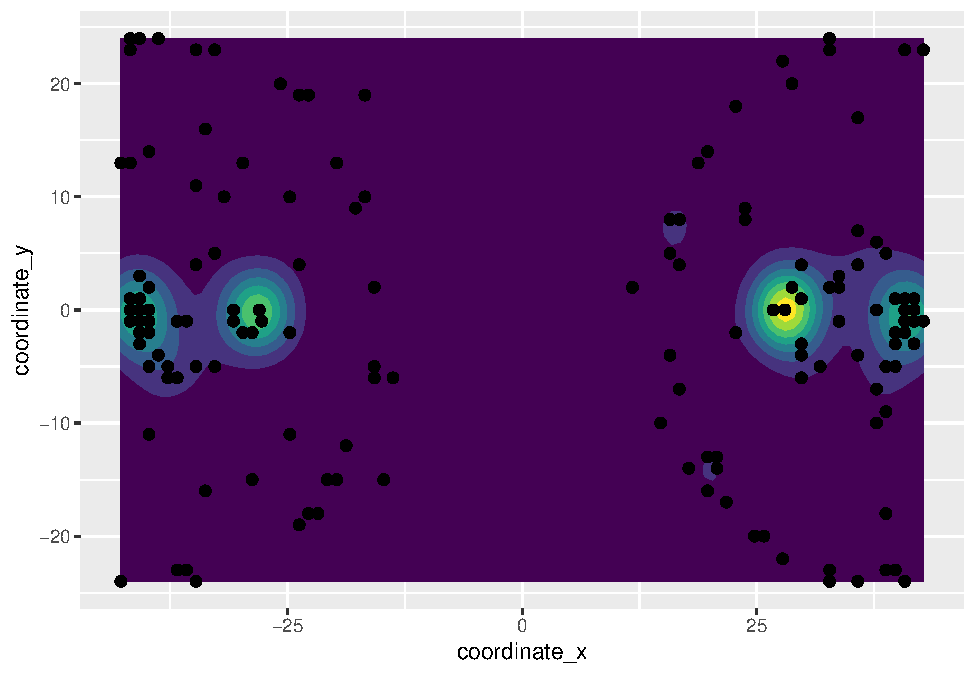
\includegraphics[keepaspectratio]{STAT442_W25_Assignment3_files/figure-latex/unnamed-chunk-9-1.pdf}}

\vspace{5cm}

\newpage

\textbf{Q9) (4 marks)} Using \texttt{geom\_basketball(league\ =\ "nba")}
in the \texttt{sportyR} package, draw a full basketball court and draw
points for shot attempts from \texttt{df\_1game\_shots} on top of the
court with \texttt{coordinate\_x} and \texttt{coordinate\_y}. Also, map
shape to \texttt{score\_type} and draw the points in Red. Put the legend
for the shape aesthetic on the bottom of the plot, and make the legend
title be ``Points''.

Hint: \texttt{geom\_basketball(league\ =\ "nba")} goes where a
\texttt{ggplot} would usually go. It just draws a basketball court, but
it doesn't take in any data, so you'll need to set the data in any
geometries that place on top.

\begin{Shaded}
\begin{Highlighting}[]
\FunctionTok{library}\NormalTok{(sportyR)}
\end{Highlighting}
\end{Shaded}

\begin{verbatim}
## Warning: package 'sportyR' was built under R version 4.4.2
\end{verbatim}

\begin{Shaded}
\begin{Highlighting}[]
\CommentTok{\#Create the plot}
\FunctionTok{geom\_basketball}\NormalTok{(}\AttributeTok{league =} \StringTok{"nba"}\NormalTok{) }\SpecialCharTok{+}
  \FunctionTok{geom\_point}\NormalTok{(}\AttributeTok{data =}\NormalTok{ df\_1game\_shots, }\FunctionTok{aes}\NormalTok{(}\AttributeTok{x =}\NormalTok{ coordinate\_x, }\AttributeTok{y =}\NormalTok{ coordinate\_y, }\AttributeTok{shape =}\NormalTok{ score\_type), }\AttributeTok{color =} \StringTok{"red"}\NormalTok{) }\SpecialCharTok{+}
  \FunctionTok{scale\_shape\_manual}\NormalTok{(}\AttributeTok{values =} \FunctionTok{c}\NormalTok{(}\DecValTok{1}\NormalTok{, }\DecValTok{2}\NormalTok{, }\DecValTok{3}\NormalTok{, }\DecValTok{4}\NormalTok{, }\DecValTok{5}\NormalTok{, }\DecValTok{6}\NormalTok{, }\DecValTok{7}\NormalTok{, }\DecValTok{8}\NormalTok{, }\DecValTok{9}\NormalTok{, }\DecValTok{10}\NormalTok{), }\AttributeTok{name =} \StringTok{"Points"}\NormalTok{) }\SpecialCharTok{+}
  \FunctionTok{theme}\NormalTok{(}\AttributeTok{legend.position =} \StringTok{"bottom"}\NormalTok{)}
\end{Highlighting}
\end{Shaded}

\pandocbounded{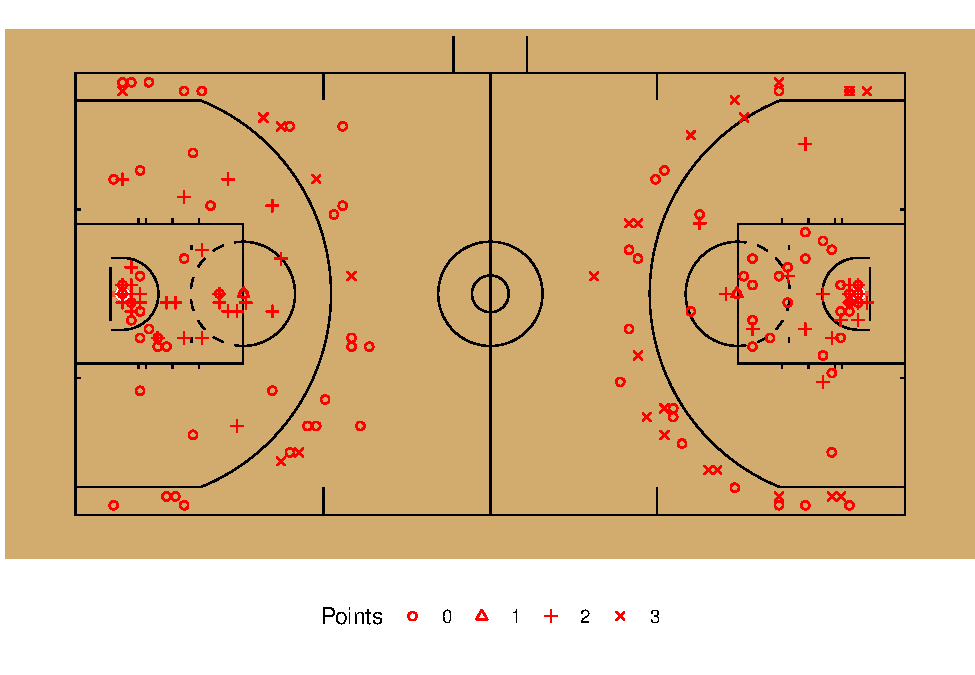
\includegraphics[keepaspectratio]{STAT442_W25_Assignment3_files/figure-latex/unnamed-chunk-10-1.pdf}}

\end{document}
